\documentclass[a4paper,10pt]{article}
\usepackage[utf8]{inputenc}
\usepackage[slovak]{babel}
\usepackage{amsmath}
\usepackage{graphicx}
\usepackage{hyperref}
\hypersetup{
    colorlinks=false,
}
\begin{document}

\title{Analytické riešenie lineárnej diferenciálnej rovnice druhého rádu s konštantnými koeficientami}
\author{Martin Dodek}
\pagestyle{plain}
\maketitle

\section{Diferenciálna rovnica}
Majme diferenciálnu rovnicu s nasledovnými vlastnosťami:
\begin{itemize}
 \item Rovnica je druhého rádu, teda obsahuje nanajvýš druhú deriváciu závislej premennej $y$
 \item Rovnica má nulovú pravú stranu. Takúto rovnicu tiež označujeme ako \emph{homogénna}.
 \item Rovnica je \emph{lineárna}, teda vystupujú v nej výlučne násobky premenných konštantami a nie iné operácie s premennými (vzájomné násobenie, umocňovanie).
 \item Koeficienty $a_i$ sú rovnako konštantné, teda sa nemenia v čase.
\end{itemize}

Rovnicu teda môžeme formulovať nasledovne:

\begin{equation}
\label{eq:diff_eq}
\ddot{y}+a_1\dot{y}+a_0y=0
\end{equation}

Riešenie diferenciálnej rovnice spočíva v nájdení \emph{funkcie} $f(t)$ popisujúcej vývoj premennej $y$ v čase.
\begin{equation*}
	y(t)=f(t)
\end{equation*}

Počiatočné podmienky (hodnoty premenných a ich derivácii v čase $t=0$) nech sú dané ako $y_0$ a $\dot{y}_0$.
Táto úloha sa potom zvykne označovať aj pojmom \emph{``initial value problem''} 

\pagebreak

\section{Charakteristická rovnica}

Charakteristická rovnica vychádza priamo z koeficientov diferenciálnej rovnice (charakteristický polynóm premennej $\lambda$) a je formulovaná nasledovne:
\begin{equation}
\label{eq:charakteristická rovnica}
	\lambda^2+a_1\lambda+a_0=0
\end{equation}

Riešením tejto charakteristickej rovnice sú dve čísla - teda korene.
Tieto korene hľadáme štandardne tak, ako v prípade kvadratickej rovnice.

Diskriminant rovnice: 
\begin{equation}
 D=a_1^2-4a_0
\end{equation}

Riešenie charakteristickej rovnice:
\label{eq:charakteristická rovnica riešenie}
\begin{equation}
 \lambda_{1,2}=\frac{-a_1\pm \sqrt{a_1^2-4a_0}}{2}
\end{equation}

Len pre pripomenutie:
\begin{equation*}
\sqrt{-1}=i
\end{equation*}

Tieto korene sú dva a sú vo všeobecnosti komplexné. 
Vzhľdaom na ich polohu v komplexnej rovine môže riešenie diferenciálnej rovnice nadobúdať nasledovné vlastnosti.

\section{Všeobecné riešenie diferenciálnej rovnice}
Podľa rozloženia koreňov charakteristického polynómu rozlišujeme nasledovné prípady:
\subsection{Rôzne reálne korene}
Riešenie diferenciálnej rovnice je v tomto prípade všeobecne definované ako súčet exponenciál.
\begin{equation}
\label{eq:riešenie reálne korene}
 y(t)=c_1e^{\lambda_1 t}+c_2e^{\lambda_2 t}
\end{equation}
Prvá derivácia riešenia bude:
\begin{equation}
\label{eq:diff riešenie reálne korene}
 \dot{y}(t)=c_1 \lambda_1 e^{\lambda_1 t}+c_2 \lambda_2 e^{\lambda_2 t}
\end{equation}


\subsection{Dvojnásobný reálny koreň}
Riešenie diferenciálnej rovnice je v tomto prípade všeobecne definované nasledovne:
\begin{equation}
\label{eq:riešenie dvojnásobný koreň}
  y(t)=c_1e^{\lambda t}+c_2 t e^{\lambda t}
\end{equation}
Prvá derivácia riešenia bude: 
\begin{equation}
\label{eq:diff riešenie dvojnásobný koreň}
 \dot{y}(t)=c_1 \lambda e^{\lambda t}+c_2e^{\lambda t} \left( 1+ t \lambda \right)
\end{equation}


\subsection{Dva komplexne združené korene}

Komplexne združený koreň má rovnakú reálnu a opačnú imaginárnu zložku.

\begin{equation*}
  \begin{array}{l}
  	\lambda_1=\lambda_a+i \lambda_b \\
  	\lambda_2=\lambda_a-i \lambda_b
  \end{array}
\end{equation*}

Riešenie diferenciálnej rovnice je v tomto prípade všeobecne definované ako súčet komplexných exponenciál.
A keďže komplexná exponenciála obsahuje periodickú zložku:
\begin{equation*}
 e^{a+bi}=e^a\left(\cos(b)+i\sin(b)\right)
\end{equation*}
Bude aj riešenie obsahovať trigonometrické funkcie.

\begin{equation}
\label{eq:riešenie komplexné korene}
  y(t)=c_1e^{\lambda_a t}\cos(\lambda_b t)+c_2e^{\lambda_a t}\sin(\lambda_b t)
\end{equation}
Prvá derivácia riešenia bude: 
\begin{equation}
\label{eq:diff riešenie komplexné korene}
 \dot{y}(t)=c_1 e^{\lambda_a t} \left( \lambda_a \cos(\lambda_b t)- \lambda_b \sin(\lambda_b t) \right) +
 c_2 e^{\lambda_a t} \left(\lambda_a \sin(\lambda_b t) + \lambda_b \cos(\lambda_b t)  \right) 
\end{equation}


\section{Riešenie s počiatočnými podmienkami}
Pre určenie koeficientov riešenia diferenciálnej rovnice $c_i$, potrebujeme poznať počiatočné podmienky.
Dosadíme nulový čas do riešenia diferenciálnej rovnice a rovnako aj do jeho prvej derivácie.
Všeobecne máme opať tri možnosti:


\subsection{Rôzne reálne korene}

Do rovníc riešenia \eqref{eq:riešenie reálne korene} a derivácie riešenia \eqref{eq:diff riešenie reálne korene} dosadíme $t=0$ .
\begin{equation}
	y(0)= c_1+c_2
\end{equation}
	
\begin{equation}
	\dot{y}(0)= c_1\lambda_1+c_2\lambda_2
\end{equation}

Zostavíme zodpovedajúcu sútavu rovníc

\begin{equation}
\label{eq:sústava pre reálne korene}
	\left(\begin{array}{c}
		y_0\\
		\dot{y}_0\\
	\end{array}\right)=
	\left(\begin{array}{c c}
	 	1 & 1 \\
	 	\lambda_1 & \lambda_1 \\
	\end{array}\right)
	\left(\begin{array}{c}
		c_1\\
		c_2\\
	\end{array}\right)
\end{equation}


\subsection{Dvojnásobný reálny koreň}
 
Do rovníc riešenia \eqref{eq:riešenie dvojnásobný koreň} a derivácie riešenia \eqref{eq:diff riešenie dvojnásobný koreň} dosadíme $t=0$ .
 
\begin{equation}
	y(0)= c_1
\end{equation}
	
\begin{equation}
	\dot{y}(0)=c_1\lambda+c_2
\end{equation}

Zostavíme zodpovedajúcu sútavu rovníc

\begin{equation}
\label{eq:sústava pre dvojnásobný koreň}
	\left(\begin{array}{c}
		y_0\\
		\dot{y}_0\\
	\end{array}\right)=
	\left(\begin{array}{c c}
	 	1 & 0 \\
	 	\lambda & 1 \\
	\end{array}\right)
	\left(\begin{array}{c}
		c_1\\
		c_2\\
	\end{array}\right)
\end{equation}


\subsection{Dva komplexne združené korene}

Do rovníc riešenia \eqref{eq:riešenie komplexné korene} a derivácie riešenia \eqref{eq:diff riešenie komplexné korene} dosadíme $t=0$ .

\begin{equation}
	y(0)=c_1
\end{equation}
	
\begin{equation}
	\dot{y}(0)=c_1\lambda_a+c_2\lambda_b
\end{equation}

Zostavíme zodpovedajúcu sútavu rovníc

\begin{equation}
\label{eq:sústava pre komplexné korene}
	\left(\begin{array}{c}
		y_0\\
		\dot{y}_0\\
	\end{array}\right)=
	\left(\begin{array}{c c}
	 	1 & 0 \\
	 	\lambda_a & \lambda_b \\
	\end{array}\right)
	\left(\begin{array}{c}
		c_1\\
		c_2\\
	\end{array}\right)
\end{equation}

\pagebreak

\section{Príklady}

\subsection{Príklad}
\begin{equation*}
\ddot{y}+3\dot{y}+2y=0 
\end{equation*}

Počiatočné podmienky nech sú dané:
\begin{equation*}
	y_0=4\quad \dot{y}_0=3
\end{equation*}

Charakteristická rovnica \eqref{eq:charakteristická rovnica} bude zostavená v tvare:
\begin{equation*}
\lambda^2+3\lambda+2=0
\end{equation*}

Riešenie charakteristickej rovnice \eqref{eq:charakteristická rovnica riešenie}
\begin{equation*}
\lambda_{1,2}=\frac{-3\pm\sqrt{9-8}}{2}
\end{equation*}

\begin{equation*}
	\lambda_2=-1 \qquad \lambda_1=-2
\end{equation*}

Získavame dva rôzne reálne korene.
Formulujeme sústavu rovníc \eqref{eq:sústava pre reálne korene}.

\begin{equation*}
	\begin{array}{c}
	c_1+c_2=4 \\
	-2c_1-c_2=3 \\
	\end{array}
\end{equation*}

Sústavu riešime elimináciou premenných

\begin{equation*}
	\begin{array}{c}
	c_1=-7 \\
	c_2=11 \\
	\end{array}
\end{equation*}

Výsledné riešenie diferenciálnej rovnice je vo forme funkcie \eqref{eq:diff riešenie reálne korene}.
\begin{equation*}
 y(t)=-7e^{-2t}+11e^{-t}
\end{equation*}

\begin{figure}[ht]
\centering
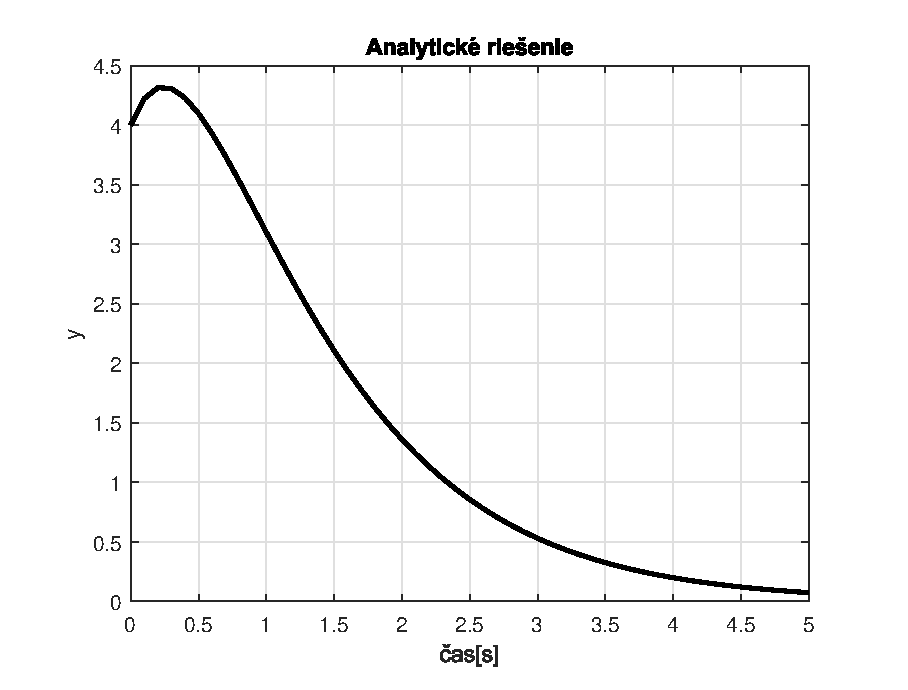
\includegraphics[width=0.7\textwidth]{graf_1} 
\caption{Časový priebeh funkcie riešenia}
\end{figure}

\pagebreak

\subsection{Príklad}

\begin{equation*}
\ddot{y}+6\dot{y}+9y=0
\end{equation*}

\begin{figure}[ht]
\centering
\includegraphics[width=0.7\textwidth]{graf_2} 
\caption{Časový priebeh funkcie riešenia}
\end{figure}

\pagebreak

\subsection{Príklad}

\begin{equation*}
\ddot{y}+2\dot{y}+10y=0
\end{equation*}

\begin{figure}[ht]
\centering
\includegraphics[width=0.7\textwidth]{graf_3} 
\caption{Časový priebeh funkcie riešenia}
\end{figure}

\end{document}